\chapter{Introduction} % Main chapter title
\label{Chapter1} % For referencing this chapter elsewhere, use \ref{Chapter1}

\section{Background}

\noindent Survival analysis is used to examine the time until the occurrence of an event, like disease relapse. A major challenge in this area is handling censored data, where the event information is incomplete. Censoring can be of different types; right-censored data is when the event has not occurred by the end of the observation period, left-censored data is when the event occurred before the study began, and interval-censored data is when the event occurred between two observed times \parencite{burzykowski_survival_2024}. To analyze such data, statistical methods have been developed.
\\\\
\noindent Non-parametric methods like the Kaplan-Meier estimator and the Logrank test do not assume any specific distribution for the time-to-event data, making them robust against mis-specifications of the event-time distribution \parencite{burzykowski_survival_2024}. Parametric methods like the Exponential and Weibull models assume a known distribution that models the time-to-event data \noindent \parencite{burzykowski_survival_2024}. They are typically more precise, at the risk of introducing bias when the assumed distribution is wrong.
\\\\
\noindent In survival analysis, understanding the survival function \( S(t)\) is crucial. The Survival Function is the statistical representation that outputs survival probabilities at various time points for given covariates (x). It quantifies the probability of an event not occurring by a certain time \(t\), effectively illustrating how the likelihood of survival decreases over time. This function is central in studies that aim to compare the effectiveness of treatments under different conditions by analyzing how quickly the events occur, such as comparing the onset times of motion sickness under varying experimental conditions.
\\\\
\noindent The Proportional Hazards Model, which can be used in both semi-parametric (Cox model) and parametric forms, is employed to estimate the hazard ratio, which is a measure of effect size regarding the time to event. An example is, that studies may compare the time until the onset of motion sickness under different conditions to assess treatment effectiveness. It is important to understand the context of discrete and continuous time models; discrete models address survival data that is categorical or not continuously distributed while the continuous model proposed by Cox, utilizes continuous data to model hazard functions \parencite{kalbfleisch_fifty_2023}. For this continuous model, estimation is based on maximizing the conditional likelihood across observed failure times, while the discrete model uses a logistic framework for estimation, treating survival as a sequence of binary outcomes. 
\\\\
\noindent Traditional statistical methods require explicit programming and often suffer from user bias in variable selection, whereas Machine Learning (ML) operates under a paradigm where algorithms autonomously identify patterns in large data sets, which potentially increases accuracy and efficiency \parencite{polce_guide_2023}. Shown below is a review \parencite{smith_scoping_2022} of methods broadly utilized in survival analysis studies, Figure \ref{fig:statsmodels}.

\begin{figure}
    \centering
    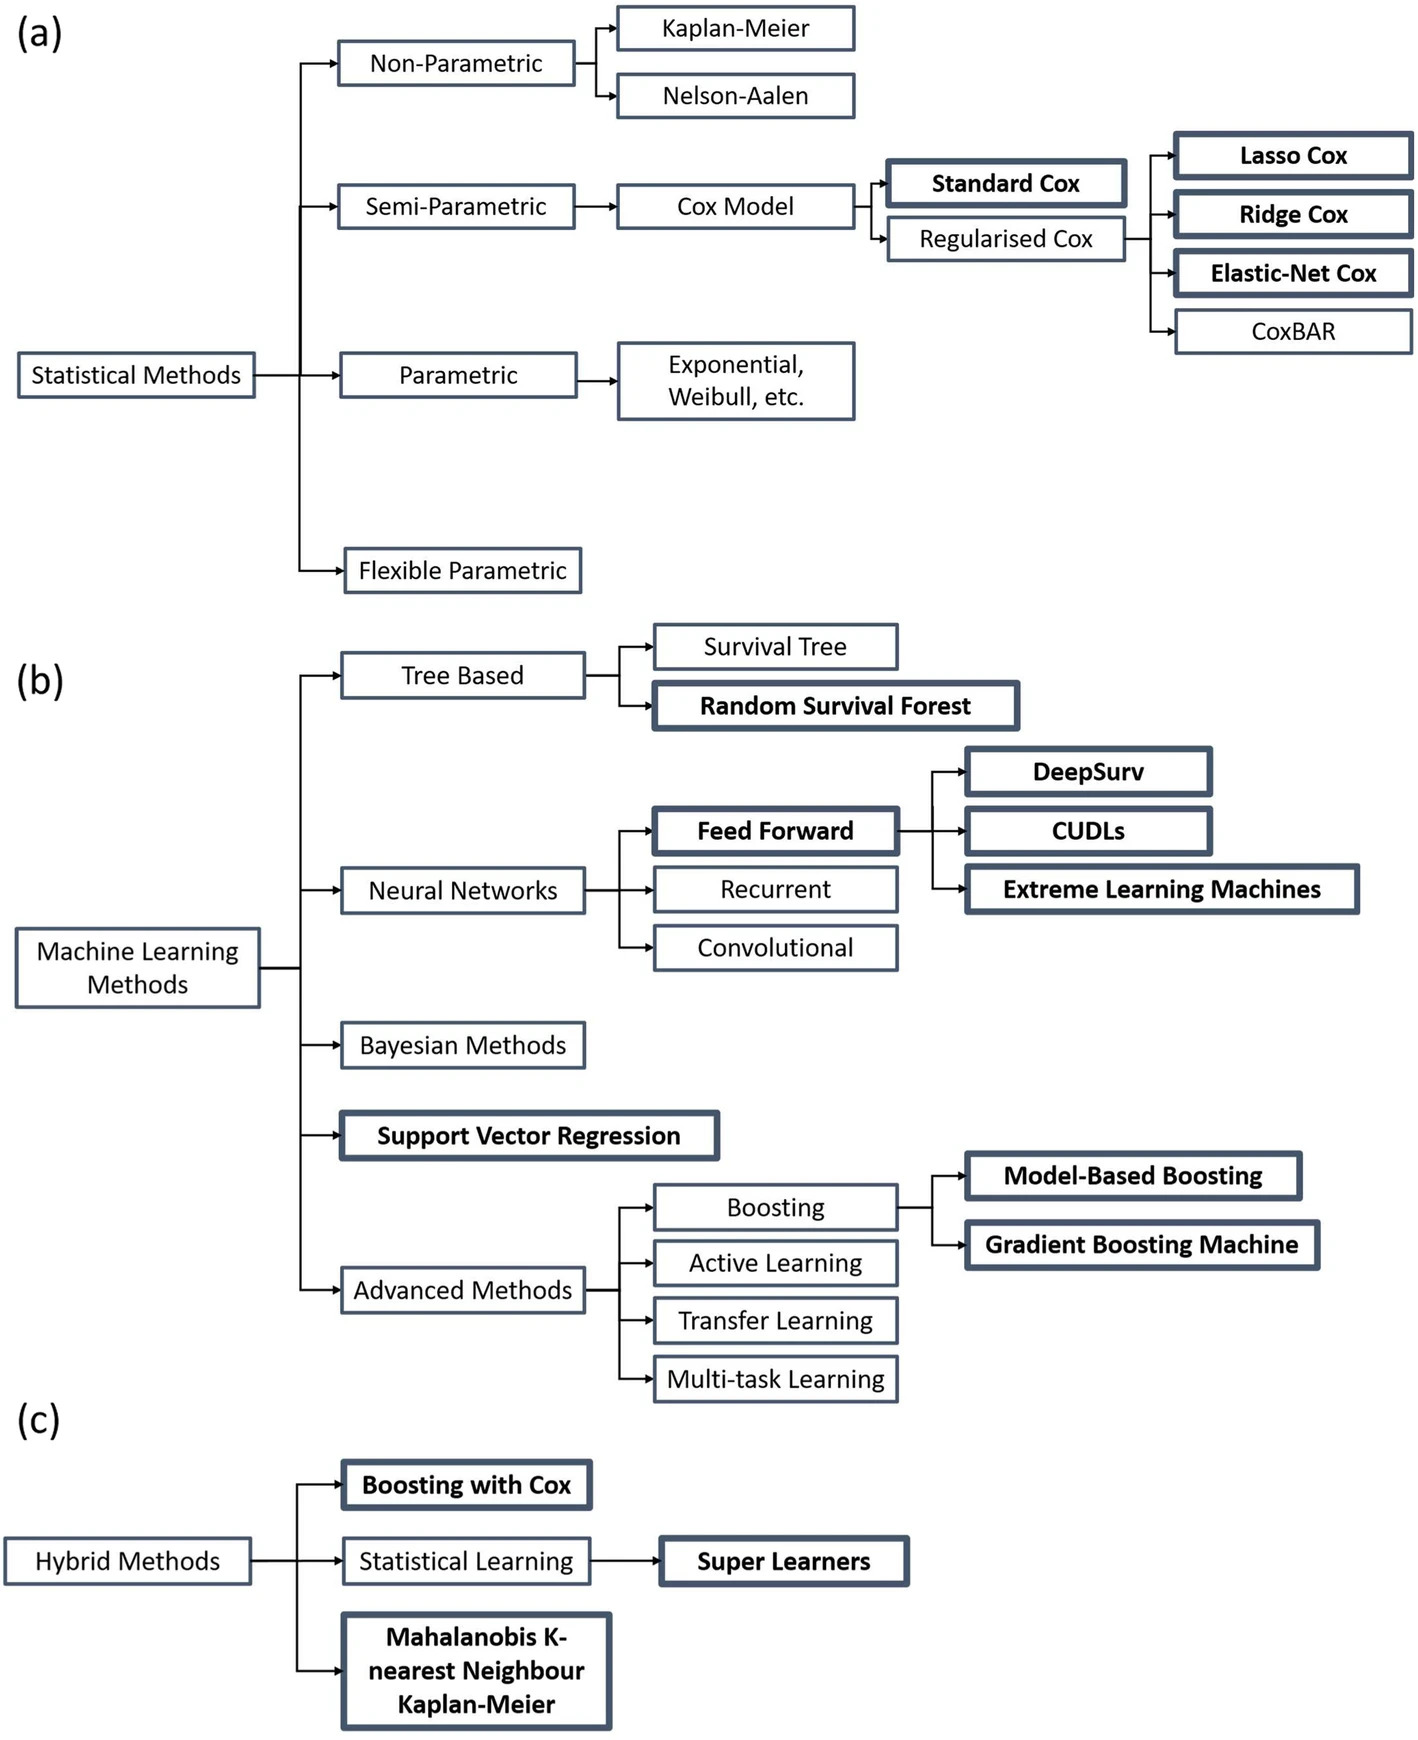
\includegraphics[scale=0.3]{Figures/ML_STATS_MODELS.jpg}
    \caption{Shows the breakdown of methods analysis preformed by \parencite{smith_scoping_2022} during a method review. The Study ran a literature selection process based on qualitative and quantitative metrics of methodology used in studies.}
    \label{fig:statsmodels}
\end{figure}

\pagebreak
\noindent Simulation studies are a crucial statistical tool used for evaluating and comparing different statistical methods, particularly when analytic solutions are hard or impossible to achieve \parencite{morris_using_2019}. These studies generate data through pseudo-random sampling from known probability distributions, enabling researchers to empirically test the behavior of statistical methods under varied scenarios. Common uses include validating new statistical methods, ensuring accuracy in mathematical models and code, and comparing the effectiveness of various approaches.
\\\\
\noindent Particularly in medical statistics, simulation studies help in designing experiments, determining sample sizes, and estimating power under specific assumptions about data generation \parencite{morris_using_2019}. Despite their widespread use, many statisticians face challenges in properly conducting simulation studies due to a lack of understanding and experience \parencite{morris_using_2019}. 
\\\\
\noindent With this proposal I present a comprehensive plan for a comparative study of survival models applied to simulated survival data, highlighting their operations, challenges, and implications.

% \noindent Pinball loss \parencite{yanagisawa_proper_2023} provides a mechanism for quantile forecasting, which is particularly useful for estimating conditional quantiles of the event time distribution. The loss function is symmetric, which allows different penalties for underestimations and overestimations.
% \begin{equation} \label{eq:pinball}
% {\text{Pinball}}(\hat{F}, y; \tau) = \begin{cases} 
% (1-\tau)(\hat{F}^{-1}(\tau) - y) & \text{if } \hat{F}^{-1}(\tau) \geq y \\
% \tau(y - \hat{F}^{-1}(\tau)) & \text{if } \hat{F}^{-1}(\tau) < y 
% \end{cases}
% \end{equation}


\section{Problem Statement}
\noindent Many studies have compared machine learning with traditional statistics, yet comprehensive simulation-based comparisons are scarce. This gap may lead to biases and sometimes questionable practices, affecting the validity of findings.

\section{Research Aims and Objectives}
\subsection{Research Aims}
\noindent Perform a comparative analysis of survival models using both simulated and real datasets to identify model robustness and effectiveness, adhering to formal frameworks \parencite{morris_using_2019} and avoiding common pitfalls outlined in the literature \parencite{pawel_pitfalls_2024}.
\subsection{Objectives}
\begin{enumerate}
    \item Source a Practical Dataset: Acquire a dataset with clear constraints and features with relevant survival data. This dataset should comply with standards \parencite{wilkinson_fair_2016}. 
    \item Run the comparative study for the survival models while adhering to the ADMEP design \parencite{morris_using_2019}
    \begin{enumerate}
        \item Apply Data Generating Methods: Utilise standard libraries to generate simulated data that closely replicate the statistical properties of the real dataset.
        \item Random Survival Forest Model: Develop and apply this model using both the real and simulated datasets.
        \item Lasso Regularized Cox Proportional Hazards Model: Similarly, develop and apply this model with both datasets.
        \item Evaluate and Visualise Predictions: Use common survival analysis metrics for evaluation and employ visualization tools from survival libraries to illustrate the results effectively.
    \end{enumerate}
    \item Document findings and interpretations along with research practices for qualitative analysis.
\end{enumerate}
 
\section{Limitations}
\begin{enumerate}
    \item \textbf{Innovation vs. Application:} This proposal does not venture to innovate on the algorithmic core of these methods. The primary focus is on the application and evaluation of established survival analysis methods and their existing extensions as documented in the literature. I seek to implement and test these pre-existing models in a new dataset context, thereby contributing to empirical evidence and practical applications rather than theoretical advancements.
    \item \textbf{Redundancy in Literature:} Furthermore, comprehensive comparative studies like those conducted by, \parencite{kurt_omurlu_comparisons_2009} \parencite{smith_scoping_2022} have already evaluated these methods extensively. These studies provide a solid foundation of knowledge regarding the performance and limitations of traditional and modified survival analysis models across various types of data.
\end{enumerate}

\section{Overview}
\noindent
In addressing the noted shortcomings in comparative simulation studies, this literature review methodically examines simulation work in segments relevant to each section of the study. I begin with an overview of the Cox method and its various extensions, illustrating how these foundational techniques are implemented. Following that, I explore proofs and extensions of the Lasso method, which builds on the base Cox method, enhancing its predictive power and flexibility. The discussion then moves to Random Survival Forests (RSF), detailing recent advancements in RSF algorithms that provide a solid reference for current implementations. Two comparative studies are highlighted; these utilize simulations to evaluate the methods mentioned above, offering insights into their practical applications and effectiveness. Finally, the last sections categorize the literature into subgroups that align with the specific components of the proposed research framework \parencite{pawel_pitfalls_2024} \parencite{morris_using_2019}, facilitating easy reference and integration into the research design and methodology in Chapter 2, ensuring a coherent and structured approach to applying these methods in this proposed study.
